% !TEX root = main.tex

\section{多元函数的积分}
\subsection{重积分基本定义}
\begin{definition}[二重积分]
设$D$是平面上可求面积的有界闭区域,$f(x,y)$定义在$D$上,用任意曲线网将$D$分成有限个可求面积的区域$\Delta\sigma_1,\Delta\sigma_2,\ldots,\Delta\sigma_n$(称为$D$的一个分法),任取$(\xi_i,\eta_i)\in\Delta\sigma_i$,作和
\[\sigma=\sum_{i=1}^nf(\xi_i,\eta_i)\Delta\sigma_i\]
记$d_i$为$\Delta\sigma_i$的直径,$\lambda=\max_{1\leq i\leq n}\{d_i\}$,若当$\lambda\to 0$时,$\sigma$的极限存在,则称$f(x,y)$在$D$可积,并称极限值为$f(x,y)$在$D$的二重积分,记为
\[\iint_Df(P)\diff\sigma\text{或}\iint_Df(x,y)\diff x\diff y\]
也即
\[\iint_Df(x,y)\diff x\diff y=\iint_Df(P)\diff\sigma=\lim_{\lambda\to 0}\sum_{i=1}^nf(\xi_i,\eta_i)\Delta\sigma_i\]
\end{definition}
\par 二重积分的基本性质与一元定积分类似(见\ref{sub:riemann}节),在此不再赘述.
涉及可积性的证明题可能还需结合定理\ref{thm:integrality}.
\begin{example}
\begin{enumerate}
	\item 证明有界闭区域上的连续函数必可积
	\item $f$在$D$上连续,$f\geq 0$且$f\not\equiv 0$,证明$\disp\int_Df\diff D>0$
	\item 证明\[f(x,y)=\begin{cases}1 & x\in\qq\\ 0 & x\notin\qq\end{cases}\]在$[0,1]\times[0,1]$上不可积
	\item $f(x)$在$[a,b]$可积,$g(y)$在$[c,d]$可积,则$f(x)g(y)$在矩形区域$D=[a,b]\times[c,d]$可积,且
	\[\iint_Df(x)g(y)\diff x\diff y=\int_a^bf(x)\diff x\int_c^dg(y)\diff y\]
\end{enumerate}
\end{example}
\begin{analysis}
\begin{enumerate}
	\item 连续函数必一致连续,则振幅可限制上界,进而对振幅与面积的乘积求和趋于$0$,可积
	\item 抽一个邻域出来,极限保号性
	\item 分别取$f(\xi_i,\eta_i)$为不同值的点,极限不同
	\item 设出$f(x),g(y)$在$\Delta\sigma_{ij}$的上下确界,分两次求和
\end{enumerate}
\end{analysis}
\begin{theorem}[富比尼(Fubini)定理]
若$f(x,y)$在矩形区域$D=[a,b]\times[c,d]$可积,且对$[a,b]$上任意$x$,含参变量积分
\[A(x)=\intabu{c}{d}{f(x,y)}{y}\]
存在,则
\[\iint_Df(x,y)\diff x\diff y=\intab{a}{b}{}\intabu{c}{d}{f(x,y)}{y}\]
即$f(x,y)$在$D$上连续,则积分次序可交换.
若$D=\{(x,y)\mid y_1(x)\leq y\leq y_2(x),a\leq x\leq b\}$,$y_1(x),y_2(x)$在$[a,b]$连续,$f(x,y)$在$D$上连续,则
\[\iint_Df(x,y)\diff x\diff y=\intab{a}{b}{}\intabu{y_2(x)}{y_1(x)}{f(x,y)}{y}\]
\end{theorem}
\par 二重积分关键确定好积分区域及积分限,有必要时注意要分段.
\par 对于三重积分的情况可以这样考虑
\begin{enumerate}
	\item 横向(平面)累加后再纵向加(注意$D_z$是变化的,即确定关于$z$的面积函数)
	\[\iiint_Vf(x,y,z)\diff x\diff y\diff z=\int_e^f\diff z\iint_{D_z}f(x,y,z)\diff x\diff y\]
	\item 纵向累加后再横向加(即投影到$D$上)
	\[\iiint_Vf(x,y,z)\diff x\diff y\diff z=\iint_D\diff x\diff y\int_{x_1(x,y)}^{x_2(x,y)}f(x,y,z)\diff z\]
\end{enumerate}
\par 由于立体空间的图像比较难想象,导致三重积分变换积分次序会比较麻烦(一共有六种情况),这时就需要逆向灵活运用上面两种方法,使三维空间的情况化归为考虑平面的情况.
\begin{example}
改变积分次序
\[I=\int_0^1\diff x\int_0^{1-x}\diff y\int_0^{x+y}f(x,y,z)\diff z\]
\end{example}
\begin{analysis}
\begin{figure}[H]
\centering
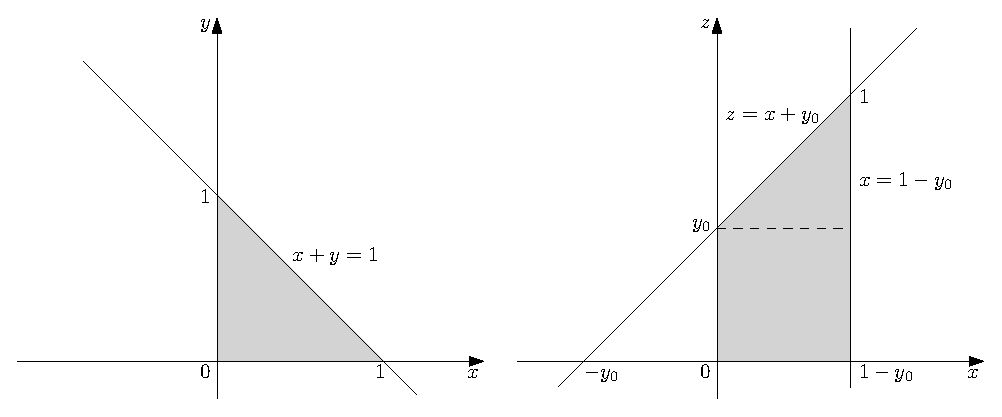
\includegraphics[width=0.6\linewidth]{fig/coordinate_eg.eps}
\end{figure}
考虑前两项,即纵向($z$方向)累加后横向加(投影到$xOy$平面上).
则可画出上图左,用二重积分的变换次序方法即可得到
\[I=\int_0^1\diff y\int_0^{1-y}\diff x\int_0^{x+y}f(x,y,z)\diff z\]
\par 再考虑后两项的次序交换,原来的后两项代表关于$x$的面积函数,则此时可以将$x$看成是常数($x_0$),这样就可以作出上图右(注意$x$的范围,以便确定直线与坐标轴交点的正负),从而又可以采用二重积分的变换方法.
注意这里需要分段求和
\[I=\int_0^1\diff y\int_0^y\diff z\int_0^{1-y}f(x,y,z)\diff x+\int_0^1\diff y\int_y^1\diff z\int_{z-y}^{1-y}f(x,y,z)\diff x\]
\par 类似地可以求得其他四种变换次序的方法.
\end{analysis}
\begin{example}
$\disp\iiint_Vxy^2z^3\diff x\diff y\diff z$,$V$由曲面$z=xy,y=x,z=0,x=1$围成
\end{example}
\begin{analysis}
对于三维空间的题目,尽可能先画出草图,确定好边界
\begin{figure}[H]
\centering
\begin{tabular}{cc}
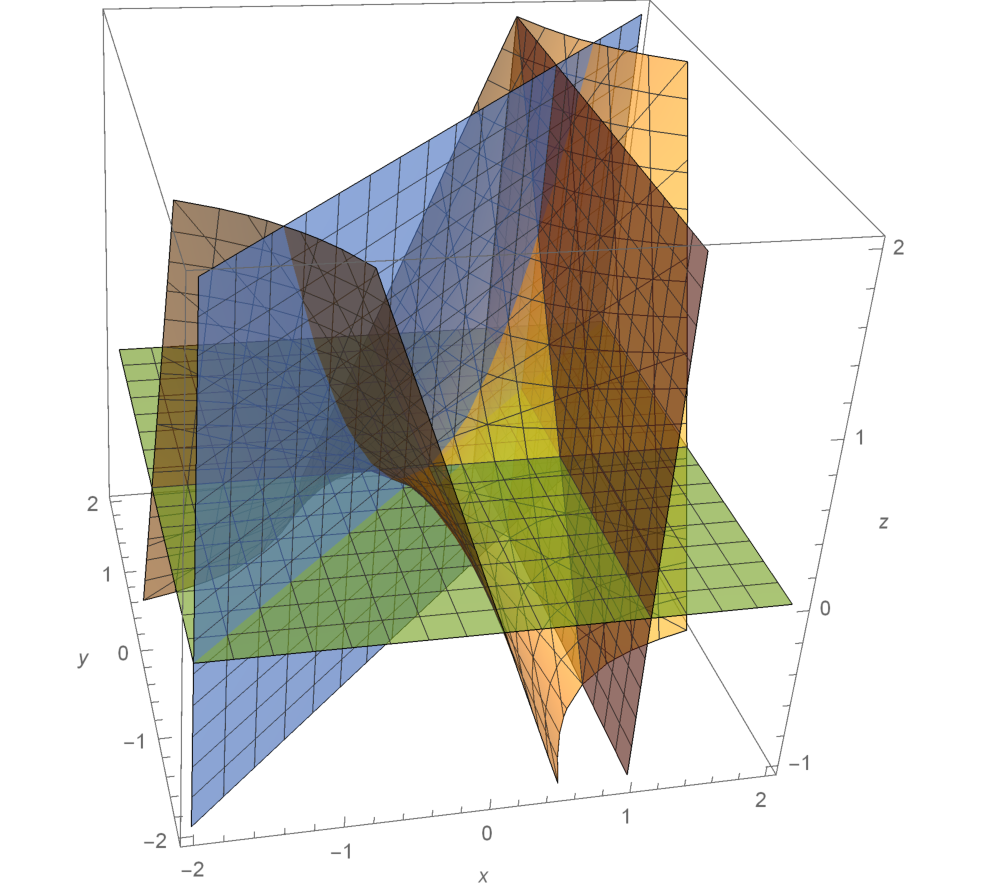
\includegraphics[width=0.4\linewidth]{fig/xy_example_side.pdf}&
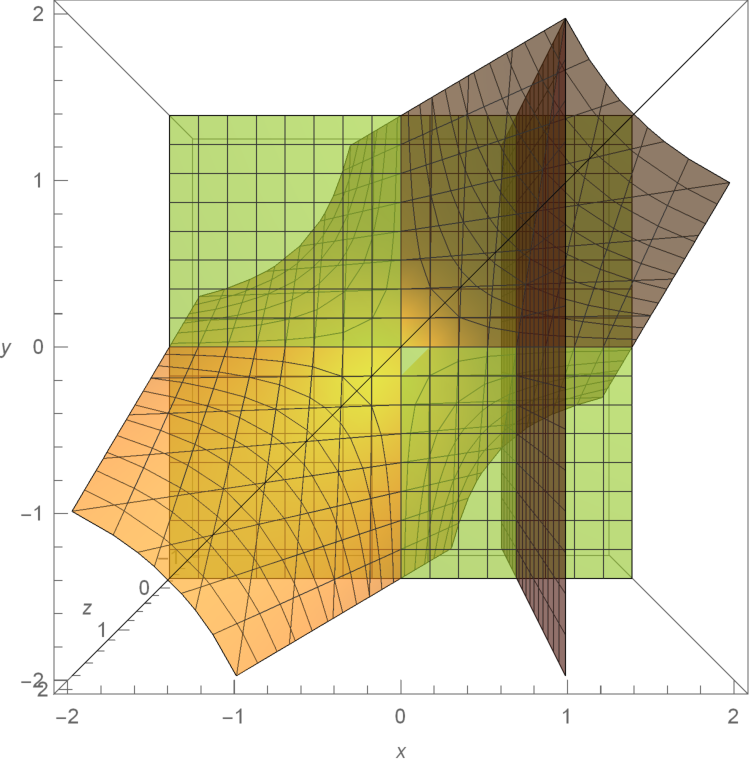
\includegraphics[width=0.3\linewidth]{fig/xy_example_front.pdf}
\end{tabular}
\end{figure}
本题中的$z=xy$形成的是一个马鞍面,在$x=0$与$y=0$两条直线上的函数值都为$0$(相当于给了一个界),且三条曲线都交于点$(1,1,1)$,进而
\[\begin{aligned}
\iiint_Vxy^2z^3\diff x\diff y\diff z&=\iint_Dxy^2\diff x\diff y\int_0^{xy}z^3\diff z\\
&=\int_0^1x\diff x\int_0^xy^2\diff y\int_0^{xy}z^3\diff z=\frac{1}{364}
\end{aligned}\]
注:此题也可出成二重积分,直接求体积($z$的两条曲线作差得到$f$)
\end{analysis}
\par 计算重积分要充分利用对称性
\begin{example}
求$\disp\iiint_V(x+y+z)\diff x\diff y\diff z,\,V:x^2+y^2+z^2\leq a^2$
\end{example}
\begin{analysis}
拆开三块进行计算,注意观察是哪项配哪项比较好算
\[\begin{aligned}
\iiint_V z\diff x\diff y\diff z&=\int_{-a}^a\diff z\iint_{D_z}z\diff x\diff y\\
&=\int_{-a}^az\diff z\iint_{D_z}\diff x\diff y\qquad\mbox{后面的二重积分直接化为面积}\\
&=\int_{-a}^az\pi(a^2-z^2)\diff z\\
&=\pi\lrp{\frac{1}{2}a^2z^2-\frac{1}{4}z^4}\Big|_{-a}^a=0
\end{aligned}\]
进而由对称性,三项均为$0$,和为$0$
\end{analysis}
\par 二重积分的几何直观是曲顶柱体的体积,或者是平面薄片的质量.
而三重积分则是四维空间曲顶柱体的体积,或者是空间物体的质量.

\subsection{重积分的变量代换}
\begin{theorem}
设变换
\[T:\begin{cases}x=\varphi(u,v)\\y=\psi(u,v)\end{cases}\]
把$Ouv$平面上由逐段光滑的闭曲线围成的区域$\Delta$一一映射为$Oxy$平面的区域$D$,且$\varphi,\psi$在$\Delta$有二阶连续偏导数,
\[J(u,v)=\frac{\partial(x,y)}{\partial(u,v)}\ne 0,\,(u,v)\in\Delta\]
而$f(x,y)$是定义在$D$上的连续函数,则
\[\iint_Df(x,y)\diff x\diff y=\iint_\Delta f(\varphi(u,v),\psi(u,v))|J(u,v)|\diff u\diff v\]
用微元的观点看,即
\[\diff S=|J(u,v)|\diff\sigma\]
注意雅可比行列式要加绝对值.
换元后$f(x,y)$会变为$f(\phi,\chi)$,而不是$f(u,v)$.
\end{theorem}
用微元的观点看会简单很多,关键确定好变换后的积分区间.
\par 三种常见的积分变换如下
\begin{enumerate}
	\item 极坐标
	\[\begin{cases}x=r\cos\theta\\y=r\sin\theta\end{cases}\implies J(r,\theta)=\frac{\partial(x,y)}{\partial(r,\theta)}=\vmat{\cos\theta & -r\sin\theta\\\sin\theta & r\cos\theta}=r\]
	\item 柱坐标变换
	\[\begin{cases}x=r\cos\theta\\y=r\sin\theta\\z=z\end{cases}\implies J(r,\theta,z)=\frac{\partial(x,y,z)}{\partial(r,\theta,z)}=\vmat{\cos\theta & -r\sin\theta & 0\\\sin\theta & r\cos\theta & 0\\ 0 & 0 & 1}=r\]
	\item 球坐标变换
	\begin{figure}[H]
	\centering
	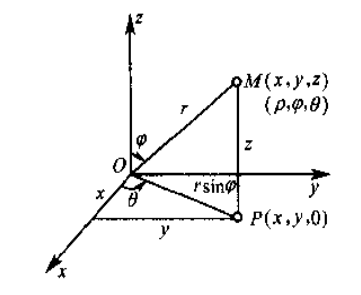
\includegraphics[width=0.3\linewidth]{fig/ball_coordinate.PNG}
	\end{figure}
	\[\begin{cases}x=r\sin\varphi\cos\theta&0\leq r<+\infty\\y=r\sin\varphi\sin\theta&0\leq\theta<2\pi\\z=r\cos\varphi & 0\leq\varphi\leq\pi\end{cases}\implies J(r,\theta,\varphi)=\vmat{\cos\theta\sin\varphi & -r\sin\theta\sin\varphi & r\cos\theta\cos\varphi\\\sin\theta\sin\varphi & r\cos\theta\sin\varphi & r\sin\theta\cos\varphi\\ \cos\varphi & 0 & -r\sin\varphi}=-r^2\sin\varphi\]
\end{enumerate}
\par 变换的目的是好算,最好变换成长方形区域,故要观察特征,抽取相同项出来,如下例.
\begin{example}
\begin{itemize}
	\item $D$由$y=4x^2,y=9x^2,x=4y^2,x=9y^2$围成
	\[T^{-1}:\;y^2=ux,x^2=vy\implies u=\frac{y^2}{x},v=\frac{x^2}{y}\]
	\item $D$由$xy=2,xy=4,y=x,y=2x$围成
	\[T^{-1}:\;u=xy,y=vx\implies u=xy,v=\frac{y}{x}\]
\end{itemize}
\end{example}

\subsection{曲线积分}
\subsubsection{第一型曲线及曲面积分}
\begin{definition}[第一型曲线积分]
设$L$为空间可求长的曲线段,$f(x,y,z)$定义在$L$上,$L$的两端点为$A,B$,依次用分点$A=A_0,A_1,\ldots,A_n=B$将$L$分为$n$小段,每小段的弧长记为$\Delta s_i$,不妨将第$i$段小弧也记为$\Delta s_i$,任取$(\xi_i,\eta_i,\zeta_i)\in\Delta s_i$,作和式
\[\sum_{i=1}^n f(\xi_i,\eta_i,\zeta_i)\Delta s_i\]
若当$\lambda=\max_{1\leq i\leq n}\{\Delta s_i\}\to 0$时上述和式极限存在,则称此极限值为$f(x,y,z)$在曲线$L$上的第一型曲线积分,记为
\[\int_Lf(x,y,z)\diff s=\lim_{\lambda\to 0}\sum_{i=1}^nf(\xi_i,\eta_i,\zeta_i)\Delta s_i\]
若$L$为光滑曲线
\[x=x(t),y=y(t),z=z(t),\alpha\leq t\leq\beta\]
$f(x,y,z)$在$L$上连续,则$f(x,y,z)$在$L$上的第一型曲线积分存在,有
\[\int_Lf(x,y,z)\diff s=\intabu{\alpha}{\beta}{f(x(t),y(t),z(t))\sqrt{{x'}^2(t)+{y'}^2(t)+{z'}^2(t)}}{t}\]
\end{definition}
由于第一型曲线积分是无向的(上限一定大于下限),故
\[\int_{\wideparen{AB}}f(x,y,z)\diff s=\int_{\wideparen{BA}}f(x,y,z)\diff s\]
\begin{definition}[第一型曲面积分]
设$S$是空间光滑曲面$z=z(x,y),(x,y)\in D$,$f(x,y,z)$是定义在$S$上的函数,对于$D$的任意分法$\Delta\sigma_i$,相应地得到$S$的分法$\Delta S_i$,任取$(\xi_i,\eta_i,\zeta_i)\in\Delta S_i$,记$\lambda=\max_{1\leq i\leq n}\{d(\Delta\sigma_i)\}$,则第一型曲面积分记为
\[\iint_S f(x,y,z)\diff S=\lim_{\lambda\to 0}\sum_{i=1}^n f(\xi_i,\eta_i,\zeta_i)\Delta S_i\]
若$D$为有界闭区域,$f(x,y,z)$在$S$上连续,则$f(x,y,z)$在曲面$S$上的第一型曲面积分存在,且
\[\iint_S f(x,y,z)\diff S=\iint_D f(x,y,z(x,y))\sqrt{1+z_x^2(x,y)+z_y^2(x,y)}\diff x\diff y\]
\end{definition}
求第一型曲面积分,关键是将曲面投影到$xOy$平面上(即$D$),即可将曲面积分变为二重积分.
\par 当曲面的参数方程不好写出时,考虑采用对称性解决.
\begin{example}
$\disp\int_Lxy\diff s$,其中$L$为球面$x^2+y^2+z^2=a^2$与平面$x+y+z=0$的交线
\end{example}
\begin{analysis}
注意观察所给式子之间的关系,有
\[-a^2=(x+y+z)^2-(x^2+y^2+z^2)=2(xy+yz+zx)\]
求三项之和的积分,注意到$x+y+z=0$过原点,故交线为大圆
\[\frac{1}{2}\int_L(-a^2)\diff s=\frac{-a^2}{2}\int_L\diff s=\frac{-a^2}{2}2\pi a=-a^3\pi\]
又注意到交线$L$关于$x,y,z$的对称性,故原式$=-\dfrac{a^3\pi}{3}$
\end{analysis}

\subsubsection{第二型曲线积分及曲面积分}
\begin{definition}[第二型曲线积分]
设向量函数$\vF(x,y,z)=P(x,y,z)\vi+Q(x,y,z)\vj+R(x,y,z)\vk$定义在空间光滑曲线弧$L$上,则
\[\begin{aligned}
\int_L\vF(x,y,z)\cdot\diff\vs&=\int_LP(x,y,z)\diff x+Q(x,y,z)\diff y+R(x,y,z)\diff z\\
&=\lim_{\lambda\to 0}\sum_{i=1}^n[P(\xi_i,\eta_i,\zeta_i)\Delta x_i+Q(\xi_i,\eta_i,\zeta_i)\Delta y_i+R(\xi_i,\eta_i,\zeta_i)\Delta z_i]\\
&=\int_a^b(Px'(t)+Qy'(t)+Rz'(t))\diff t
\end{aligned}\]
\end{definition}
若$L$为闭曲线,则记
\[\oint_LP\diff x+Q\diff y+R\diff z\]
此时积分与起点选择无关,只与曲线$L$的方向有关.
\par 注意积分公式中定积分的\textbf{下限}总是对应有向曲线段的\textbf{起点},\textbf{上限}总是对应有线曲线段的\textbf{终点}.
路径不同,积分值可能不同.
\[\int_{\wideparen{AB}}\vF\cdot \diff\vs=\int_{\arc{AB}}\vF\cdot\vtau\diff d\]
其中,$\vtau$是与$\arc{AB}$方向一致的单位切向量,用分量表示即为
\[(\diff x,\diff y,\diff z)=(\cos\alpha,\cos\beta,\cos\gamma)=(\frac{\diff x}{\diff s},\frac{\diff y}{\diff s},\frac{\diff z}{\diff s})\]
\par 涉及切向量/法向量的式子大多用\textbf{本性方程}进行推导,下面是一例关于本性方程的应用.
\begin{example}
设$P,Q,R$在$L$上连续,$L$为光滑弧段,弧长为$l$,证明
\[\left|\int_LP\diff x+Q\diff y+R\diff z\right|\leq Ml\]
其中$M=\max_{(x,y,z)\in L}\{\sqrt{P^2+Q^2+R^2}\}$
\end{example}
\begin{analysis}
取弧长$s$为参数,则$L$的本性方程为
\[\begin{cases}
x=x(s)\\
y=y(s)&0\leq s\leq l\\
z=z(s)
\end{cases}\]
进而有
\[\begin{aligned}
\Big|\int_LP\diff x+&Q\diff y+R\diff z\Big|=
\left|\int_0^lP(x(s),y(s),z(s))\diff x(s)+\int_0^lQ(x(s),y(s),z(s))\diff y(s)+\int_0^lR(x(s),y(s),z(s))\diff z(s)\right|\\
&\leq \int_0^l\left|P(x(s),y(s),z(s))\diff x(s)+Q(x(s),y(s),z(s))\diff y(s)+R(x(s),y(s),z(s))\diff z(s)\right|\quad\mbox{绝对值不等式}\\
&\leq \int_0^l\sqrt{P^2+Q^2+R^2}\sqrt{\diff x^2+\diff y^2+\diff z^2}\quad\mbox{Cauchy不等式}\\
&\leq M\int_0^l\diff s=Ml
\end{aligned}\]
\end{analysis}
\begin{definition}[第二型曲面积分]
设向量函数$\vF(x,y,z)=P(x,y,z)\vi+Q(x,y,z)\vj+R(x,y,z)\vk$定义在空间光滑光滑双侧曲面$S$上,则
\[\begin{aligned}
\iint_S\vF(x,y,z)\cdot\diff\vS&=\iint_SP(x,y,z)\diff y\diff z+Q(x,y,z)\diff z\diff x+R(x,y,z)\diff x\diff y\\
&=\lim_{\lambda\to 0}\sum_{i=1}^n[P(\xi_i,\eta_i,\zeta_i)\Delta S_i\cos\alpha_i+Q(\xi_i,\eta_i,\zeta_i)\Delta S_i\cos\beta_i+R(\xi_i,\eta_i,\zeta_i)\Delta S_i\cos\gamma_i]\\
&=\iint_S(P\cos\alpha+Q\cos\beta+R\cos\gamma)\diff S\\
&=\pm\iint_D (P,Q,R)\cdot\lrp{\pd{(y,z)}{(u,v)},\pd{(z,x)}{(u,v)},\pd{(x,y)}{(u,v)}}\diff u\diff v\\
&=\iint_D\pm P\left|\pd{(y,z)}{(u,v)}\right|\diff y\diff z\pm Q\left|\pd{(z,x)}{(u,v)}\right|\diff z\diff x\pm R\left|\pd{(x,y)}{(u,v)}\right|\diff u\diff v
\end{aligned}\]
这里的$(\cos\alpha,\cos\beta,\cos\gamma)$是法向量与坐标轴的夹角
\end{definition}
\par 曲面的侧由$\cos\gamma$的正负决定,若$\vn$与$z$轴正向夹角为锐角,则为曲面的上侧,否则为曲面的下侧.
\begin{theorem}
设$R(x,y,z)$在光滑曲面$S:z=z(x,y),(x,y)\in D$上连续,则
\[\iint_SR(x,y,z)\diff x\diff y=\sgn(\cos\gamma)\iint_DR(x,y,z(x,y))\diff x\diff y\]
\end{theorem}

\subsubsection{各类积分之间的联系}
\begin{definition}[简单闭曲线]
封闭无交叉点的曲线
\end{definition}
\begin{definition}[连通区域]
平面区域$D$上任何一条封闭曲线都可以不经过$D$以外的点而连续地收缩为属于$D$的一点,则称$D$为平面单连通区域,否则为复连通区域
\end{definition}
\par 规定区域$D$的边界$L$的正方向是指沿$L$行走时,所围的区域$D$总在左侧;规定了正方向的边界记为$L^+$.
\par 国外的教材均不对第一第二型积分进行区分,一般提到线积分或面积分都是指第二型积分,而第一型积分则是标量场意义下的线积分或面积分.
\begin{center}
\begin{tabular}{|c|c|c|c|}\hline
第一型曲线积分(一线) & 标量场 & $\disp\int_\mL f(x,y,z)\diff l$ & 线密度\\\hline
第二型曲线积分(二线) & 矢量场 & $\disp\int_\mL\vF(x,y,z)\cdot\diff\vl$ & 变力做功\\\hline
第一型曲面积分(一面) & 标量场 & $\disp\iint_\mS f(x,y,z)\diff S$ & 面密度\\\hline
第二型曲面积分(二面) & 矢量场 & $\disp\iint_\mS\vF(x,y,z)\cdot\diff\vS$ & 流量\\\hline
\end{tabular}
\end{center}
\par 牛顿-莱布尼茨公式在高维空间的推广,即将内部积分转化为边界积分
\begin{theorem}[格林(Green)公式]
设$D$由逐段光滑闭曲线$L$围成的平面单连通区域,函数$P(x,y),Q(x,y)$在$D$上有一阶\textbf{连续}偏导数,则
\[\iint_D\lrp{\pd{Q}{x}-\pd{P}{y}}\diff x\diff y=\iint_D\vmat{\pd{}{x}&\pd{}{y}\\P&Q}=\oint_{L^+}P\diff x+Q\diff y\]
\end{theorem}
格林公式运用时注意补弧或者挖洞.
\par 平面区域$D$的面积
\[|D|=\iint_D\diff x\diff y=\frac{1}{2}\oint_Lx\diff y-y\diff x\]
\begin{theorem}[高斯(Gauss)公式]
设空间区域$V$由分片光滑的双侧封闭曲面$S$围成,函数$P(x,y,z),Q(x,y,z),R(x,y,z)$在$V$及$S$上有一阶\textbf{连续}偏导数,则
\[\iiint_V\lrp{\pd{P}{x}+\pd{Q}{y}+\pd{R}{z}}\diff x\diff y\diff z=\oiint_{S^+}P\diff y\diff z+Q\diff z\diff x+R\diff x\diff y\]
其中$S^+$为曲面$S$的外侧
\end{theorem}
\begin{theorem}[斯托克斯(Stokes)公式]
若光滑曲面$S$的边界为光滑曲线$L$,函数$P(x,y,z),Q(x,y,z),R(x,y,z)$在曲面$S$及曲线$L$上有连续一阶偏导数,则
\[\begin{aligned}
\oint_{\mL^+} P\diff x+Q\diff y+R\diff z&=\iint_{S^+}\lrp{\pd{R}{y}-\pd{Q}{z}}\diff y\diff z+\lrp{\pd{P}{z}-\pd{R}{x}}\diff z\diff x+\lrp{\pd{Q}{x}-\pd{P}{y}}\diff x\diff y\\
&=\iint_S\vmat{\diff y\diff z&\diff z\diff x&\diff x\diff y\\\pd{}{x}&\pd{}{y}&\pd{}{z}\\P&Q&R}\\
&=\iint_S\vmat{\cos\alpha&\cos\beta&\cos\gamma\\\pd{}{x}&\pd{}{y}&\pd{}{z}\\P&Q&R}\diff S
\end{aligned}\]
\end{theorem}

结合场论的符号(见第\ref{sec:field}章),可以得到以下这张关系图.
其中,$\vtau$是与$\mL$方向一致的\textbf{单位切向量},$\vn$是与$\mS$同侧的\textbf{单位法向量},且有
\[\begin{aligned}
\diff\vl&=\vtau\diff l=(\cos(\vtau,x),\cos(\vtau,y),\cos(\vtau,z))\diff l=(\diff x,\diff y,\diff z)\\
\diff\vS&=\vn\diff S=(\cos(\vn,x),\cos(\vn,y),\cos(\vn,z))\diff S=(\diff y\diff z,\diff z\diff x,\diff x\diff y)
\end{aligned}\]
\begin{figure}[H]
\centering
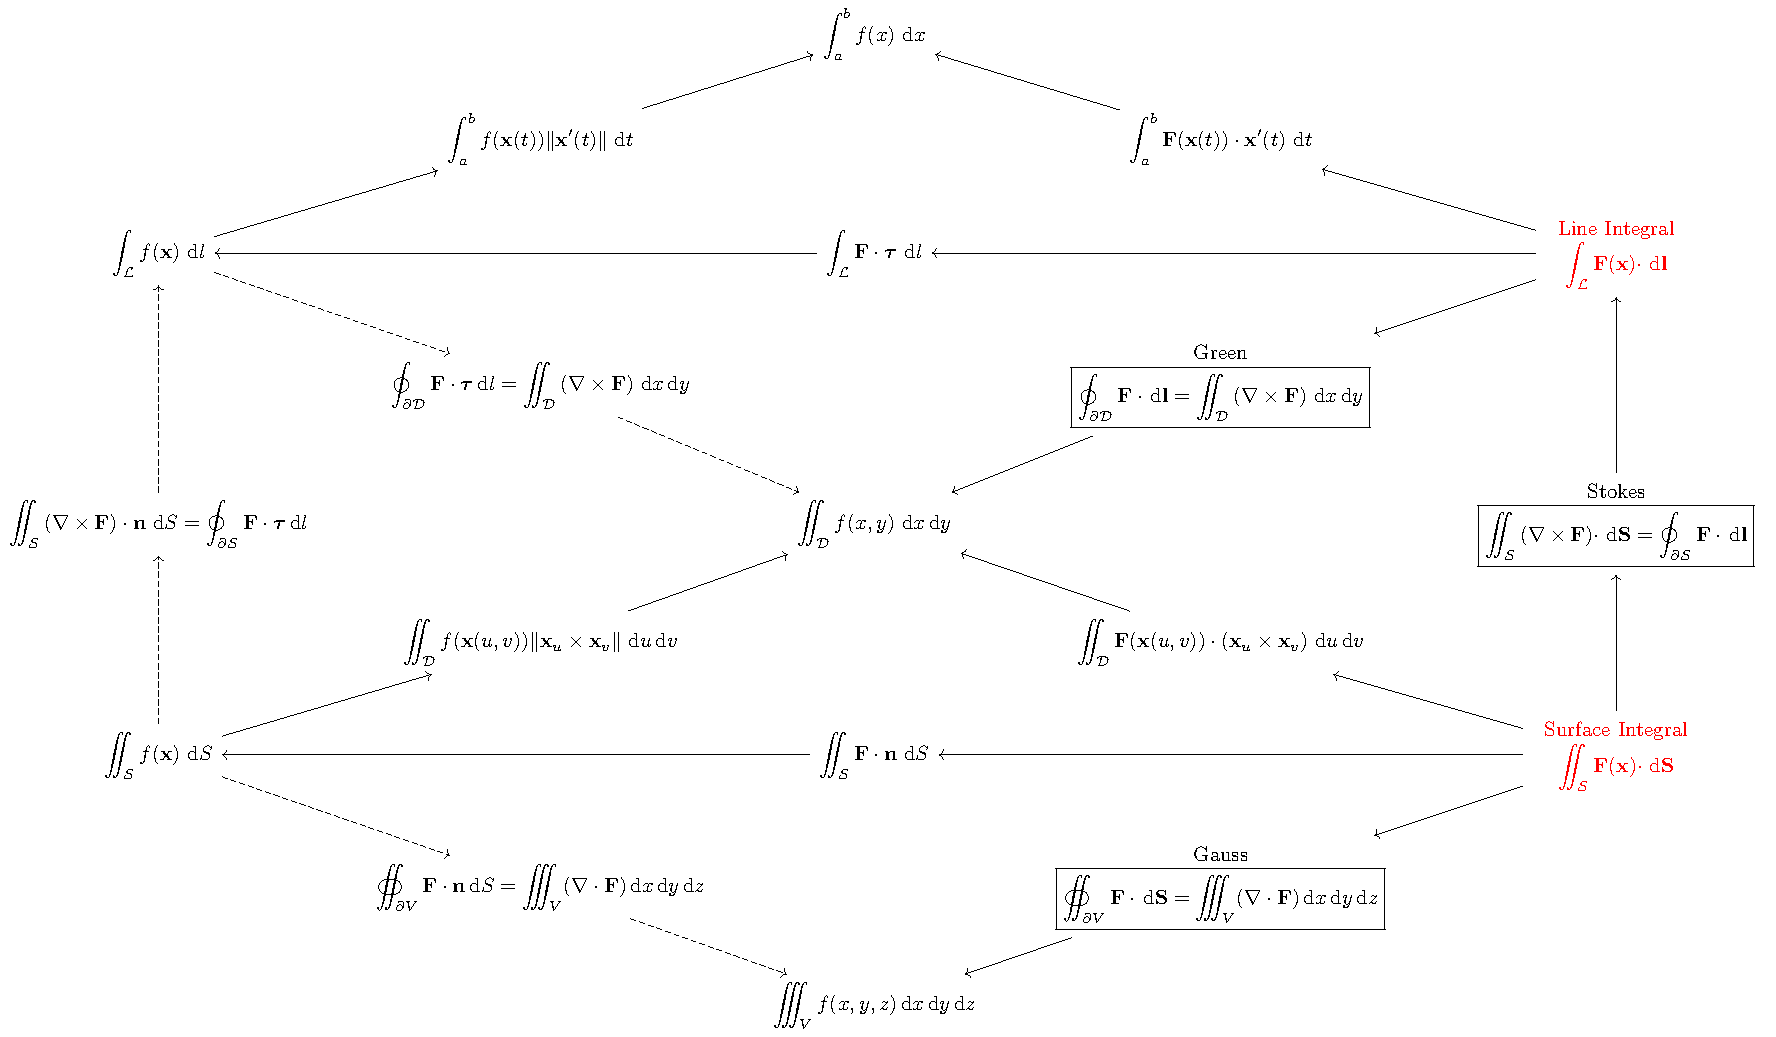
\includegraphics[width=\linewidth]{fig/multivar-integral-relationship.pdf}
\end{figure}
\par 三大公式用外微分形式表示,如$\partial\mD$表示$\mD$区域的边界.
\par 同时注意下式的关系成立,是法向量,但\textbf{不是单位}法向量(见\ref{subsubsec:surface_area}节)
\[\vx_u\times\vx_v=\lrp{\pd{(u,v)}{(y,z)},\pd{(u,v)}{(z,x)},\pd{(u,v)}{(x,y)}}\]

\subsubsection{积分与路径无关}
\begin{theorem}
设$D$为平面单连通区域,函数$P(x,y)$,$Q(x,y)$在$D$上有连续偏导数,则下列四个命题等价
\begin{enumerate}
	\item 沿$D$中任一逐段光滑闭曲线$L$,有
	\[\oint_LP\diff x+Q\diff y=0\]
	\item 对$D$中任一逐段光滑曲线$L$,曲线积分
	\[\int_LP\diff x+Q\diff y\]
	与路径无关,只与$L$的起点和终点有关
	\item 微分式$P\diff x+Q\diff y$在$D$内是某函数$u(x,y)$的全微分,即有
	\[\diff u=P\diff x+Q\diff y\]
	\item 在$D$内每一点有
	\[\vmat{\vi&\vj\\\pd{P}{y}&\pd{Q}{x}}=0\]
\end{enumerate}
\end{theorem}
\begin{theorem}[奇点]
关于奇点的结论
\begin{enumerate}
	\item 对$D$内任意一条不包围奇点的闭曲线$L$,有
	\[\oint_LP\diff x+Q\diff y=0\]
	\item 环绕某一奇点的任意两条简单闭曲线$L_1,L_2$的积分相等,即
	\[\oint_{L_1}P\diff x+Q\diff y=\oint_{L_2}P\diff x+Q\diff y\]
	这个公共值称为该奇点的循环常数
	\item 环绕某一奇点$n$圈的光滑闭曲线$L$,其中$n_1$圈为正向,$n_2$圈为负向,$n_1+n_2=n$,则积分
	\[I=\oint_LP\diff x+Q\diff y\]
	等于该点循环常数的$n_1-n_2$倍
	\item 若不自相交光滑闭曲线$L$包围了$k$个奇点,则沿$L$正向的积分
	\[I=\oint_LP\diff x+Q\diff y\]
	等于这$k$个奇点循环常数之和
\end{enumerate}
\end{theorem}
\begin{definition}[原函数]
若$\diff u(x,y)=P(x,y)\diff x+Q(x,y)\diff y$,则称$u(x,y)$为$P\diff x+Q\diff y$的原函数
\end{definition}
\par 注意看积分区域包不包含奇点,若包含则需分类讨论
\begin{example}
设$L$为不经过$(-2,0)$和$(2,0)$点的简单闭曲线,求
\[\begin{aligned}
I&=\oint_L\left[\frac{y}{(x-2)^2+y^2}+\frac{y}{(x+2)^2+y^2}\right]\diff x\\
&+\left[\frac{2-x}{(2-x)^2+y^2}+\frac{-(2+x)}{(x+2)^2+y^2}\right]\diff y
\end{aligned}\]
\end{example}
\begin{analysis}
依题意有
\[\begin{aligned}
P(x,y)&=\frac{y}{(x-2)^2+y^2}+\frac{y}{(x+2)^2+y^2}\\
Q(x,y)&=\frac{2-x}{(2-x)^2+y^2}+\frac{-(2+x)}{(x+2)^2+y^2}
\end{aligned}\]
可求得$A(-2,0),B(2,0)$为奇点,当$(x,y)\ne A,B$时$\pd{P}{y}=\pd{Q}{x}$.
设$L$包含的区域为$D$
\begin{enumerate}
	\item 若$D$不包含$A,B$,则由格林公式
	\[I=\iint_D\lrp{\pd{P}{y}-\pd{Q}{x}}=0\]
	\item 若$D$包含$A$和$B$,则分别以$A,B$为圆心,以很小的正数$\eps$为半径作圆$r_1,r_2$,使得$r_1,r_2\in D$且$r_1\cap r_2=\varnothing$,有积分等于奇点循环常数之和,即
	\[I=\oint_{r_1}P\diff x+Q\diff y+\oint_{r_2}P\diff x+Q\diff y\]
	设
	\[\begin{aligned}
	P_1&=\frac{y}{(x-2)^2+y^2}\qquad&Q_1&=\frac{2-x}{(2-x)^2+y^2}\\
	P_2&=\frac{y}{(x+2)^2+y^2}\qquad&Q_2&=\frac{-(2+x)}{(x+2)^2+y^2}
	\end{aligned}\]
	在$r_1$包围的区域$D_1$内,$P_1,Q_1$均有连续偏导数,且$\pd{P_1}{y}=\pd{Q_1}{x}$;\\
	在$r_2$包围的区域$D_2$内,$P_2,Q_2$均有连续偏导数,且$\pd{P_2}{y}=\pd{Q_2}{x}$;
	故有
	\[\begin{aligned}
	I&=\oint_{r_1}P_2\diff x+Q_2\diff y+\oint_{r_2} P_1\diff x+Q_1\diff y\\
	&=\frac{1}{\eps^2}\oint_{r_1}y\diff x-(2+x)\diff y+\frac{1}{\eps^2}\oint_{r_2}y\diff x+(2-x)\diff y\\
	&=\frac{1}{\eps^2}\iint_{D_1}(-2)\diff x\diff y+\frac{1}{\eps^2}\iint_{D_2}(-2)\diff x\diff y\qquad\mbox{格林公式}\\
	&=-4\pi
	\end{aligned}\]
	\item 若$D$只含$A,B$中其中一个,同上理可得$I=-2\pi$
\end{enumerate}
综上,
\[I=\begin{cases}0&\text{$D$不含$A,B$}\\-2\pi&\text{$D$中只含$A,B$中任一个}\\-4\pi&\text{$D$包含$A,B$}\end{cases}\]
\end{analysis}